\documentclass[10pt]{beamer}

\usetheme[progressbar=frametitle]{metropolis}
\usepackage{appendixnumberbeamer}

\usepackage{listings}

\usepackage{booktabs}
\usepackage[scale=2]{ccicons}

\usepackage{pgfplots}
\usepgfplotslibrary{dateplot}

\usepackage{xspace}
\newcommand{\themename}{\textbf{\textsc{metropolis}}\xspace}
\lstset{literate=
    {->}{{$\rightarrow\;$}}1
    {=>}{{$\Rightarrow\;$}}1}

\title{Generic programming in Scala}
\subtitle{[Superfunky library name here]}
% \date{\today}
\date{}
\author{Carlos Tomé Cortiñas
\and Matthew Swart
\and Renate Eilers}
\institute{Department of Information and Computing Sciences, Utrecht University}
% \titlegraphic{\hfill\includegraphics[height=1.5cm]{logo.pdf}}

\begin{document}

\maketitle

\begin{frame}{Table of contents}
  \setbeamertemplate{section in toc}[sections numbered]
  \tableofcontents[hideallsubsections]
\end{frame}

\section{An introduction to generic programming}

\begin{frame}[fragile]
\frametitle{Generic programming -- Why?}

Do you ever find yourself writing variations of the same program over and over?

% Consider the following two functions for calculating size of a list and a tree
% They look different on the surface, but in essence they do the same:
% both recursively calculate the size of the substructures of what they are passed, and then put these results together
\begin{columns}
\begin{column}{.40\textwidth}
\begin{lstlisting}[language=Haskell,basicstyle=\ttfamily\scriptsize]
data List a = Cons a (List a)
            | Nil

size :: List a -> Int
size Nil = 0
size (Cons x xs) = 1 + size xs
\end{lstlisting}
\end{column}
\begin{column}{.48\textwidth}
\begin{lstlisting}[language=Haskell,basicstyle=\ttfamily\scriptsize]
data Tree a = Node (Tree a) (Tree a)
            | Leaf a

size :: Tree a -> Int
size (Leaf n) = 1
size (Node l r) = 1 + size l + size r
\end{lstlisting}
\end{column}
\end{columns}

Write functions on the {\color{green}\emph{structure}} of datatypes rather than on concrete instantiations.
\end{frame}

\begin{frame}[fragile]
\frametitle{Generic programming -- What?}
Most datatypes can be represented by combination of {\color{blue}\emph{basic types}} such as \textbf{units}, \textbf{sum} and \textbf{product}:

\begin{columns}
\begin{column}{.40\textwidth}
\begin{lstlisting}[language=Haskell,basicstyle=\ttfamily\scriptsize]
data List a = Nil | Cons a (List a)
\end{lstlisting}
\vspace{-3pt}vs.
\begin{lstlisting}[language=Haskell,basicstyle=\ttfamily\scriptsize,mathescape]
data RList a = () :+: (a :$\times$: (List a))
\end{lstlisting}
\end{column}
\begin{column}{.35\textwidth}
\begin{lstlisting}[language=Haskell,basicstyle=\ttfamily\scriptsize,mathescape]
data () = ()
data a :+: b = Inl a | Inl b
data a :$\times$: b = a :$\times$: b
\end{lstlisting}
\end{column}
\end{columns}
A program written to work on these standard types can be used on \underline{\emph{any}} datatype provided a conversion between both types is supplied!

\begin{lstlisting}[language=Haskell,basicstyle=\ttfamily\scriptsize]
data Iso a b = Iso {from :: a -> b, to :: b -> a}

fromList :: List a -> RList a
toList   :: RList a -> List a
\end{lstlisting}

\end{frame}

\section{Shapeless}
\begin{frame}[fragile]
 Representation of case classes/sealed traits based on HList and Coproducts
\begin{lstlisting}[language=Scala,basicstyle=\ttfamily\scriptsize]
sealed trait Shape
case class Rectangle(width: Double, height: Double) extends Shape
case class Circle(radius: Double) extends Shape

val gen = Generic[Shape]
gen: shapeless.Generic[Shape]{type Repr = shapeless.:+:
                      [Rectangle,shapeless.:+:[Circle,shapeless.CNil]]}
\end{lstlisting}
The pattern:
\begin{lstlisting}[language=Scala,basicstyle=\ttfamily\scriptsize]
trait Eq[A] {
  def eq(x : A, y : A) : Boolean
}
implicit val hnilEq: Eq[HNil] = {..}
implicit def hlistEq[H, T <: HList](..) = {..}

implicit val cnilEq : Eq[CNil] = {..}
implicit def coproductEq[H, T <: Coproduct](..) = {..}

implicit def genericEq[A, R](
    implicit
      gen: Generic.Aux[A, R],
      env: Lazy[Eq[R]]
  ) : Eq[A] = {..}
\end{lstlisting}

\end{frame}
% Introduce shapeless, what is their approach?

\section{EMGM}
\begin{frame}
\frametitle{Criteria for generic programming libraries}
% Many Haskell libraries for GP exist
% Each has its own set of pros and cons
% A recent study has compared some of the libraries, the results are presented in this table
% Explain some of the criteria
% Show that EMGM generally scores well, say that Shapeless is based on SYB
% EMGM complements SYB, hence we chose it
\begin{center}
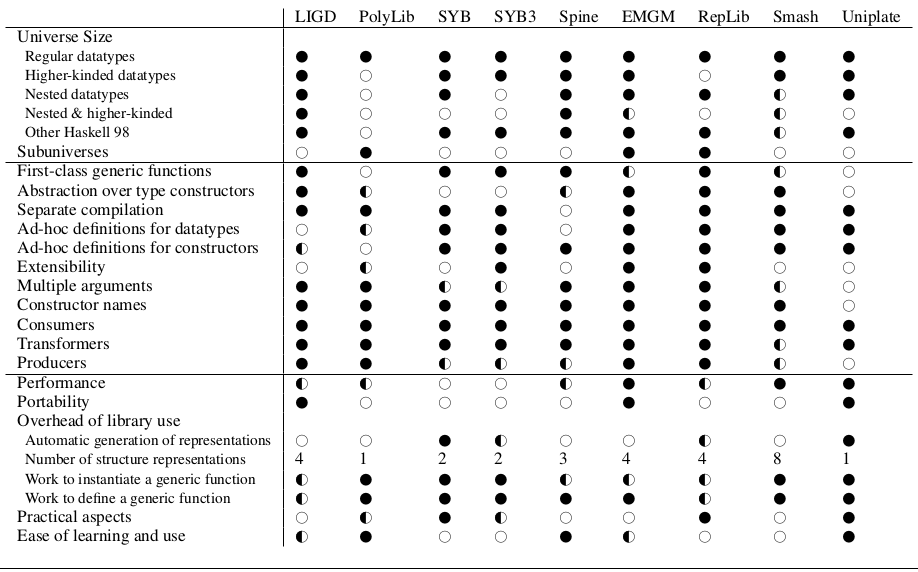
\includegraphics[scale=0.35]{Images/Comparisons.png}
\end{center}
\end{frame}

\begin{frame}[fragile]
\frametitle{EMGM I}
\textbf{E}xtensible and \textbf{M}odular \textbf{G}enerics for the \textbf{M}asses.
\vspace{30pt}

Functions are implemented using the \texttt{Generic} class:\\

\begin{center}
\begin{lstlisting}[language=Haskell,basicstyle=\ttfamily\scriptsize,mathescape]
class Generic g where
    unit :: g ()
    plus :: g a -> g b -> g (a :+: b)
    prod :: g a -> g b -> g (a :$\times$: b)
    int  :: g Int
    view :: Iso b a$\footnote{The type \texttt{Iso b a} signifies an isomorphism between the types \texttt{a} and \texttt{b}.}$ -> g a -> g b
\end{lstlisting}
\end{center}
\end{frame}

\begin{frame}[fragile]
\frametitle{EMGM II}
 Type representations are encoded in the \texttt{Rep} class.

\vspace{30pt}



\begin{lstlisting}[language=Haskell,basicstyle=\ttfamily\scriptsize,mathescape]
class Rep g a where
  rep :: g a

instance (Generic g) => Rep g Int where
  rep = int
\end{lstlisting}



\end{frame}


\begin{frame}[fragile]
\frametitle{EMGM III}
To write a generic function we define a type and make it an instance of \texttt{Generic}. As an example, let's define a generic encoding function:
\begin{lstlisting}[language=Haskell,basicstyle=\ttfamily\scriptsize,mathescape]
newtype Encode a =  Enc {enc :: a -> [Bit]}

instance Generic Encode where
    unit       = Enc (const [])
    plus a b   = Enc ($\lambda$ x -> case x of
                   Inl l -> 0:enc a l
                   Inr r -> 1:enc b r
    prod a b   = Enc ($\lambda$ (x :+: y) ->
                   enc a x ++ enc b y
    int        = Enc encodeInt
    view iso a = Enc ($\lambda$ x -> enc a (from iso x)}
\end{lstlisting}

\end{frame}


\section{Implementation}
\begin{frame}[fragile]
\frametitle{Converting Haskell code to Scala: type classes}
Haskell's type classes can be simulated by Scala's traits:

\begin{columns}
\begin{column}{.35\textwidth}
\begin{lstlisting}[language=Haskell,basicstyle=\ttfamily\scriptsize,mathescape]
class Generic g where
    unit :: g Unit
    plus :: g a -> g b ->
      g (a :+: b)
    prod :: g a -> g b ->
      g (a :$\times$: b)
    int  :: g Int
    view :: Iso b a ->
      g a -> b a
\end{lstlisting}
\end{column}
\begin{column}{.60\textwidth}
\begin{lstlisting}[language=Scala,basicstyle=\ttfamily\scriptsize,mathescape]
trait Generic[G[_]] {
    def unit: G[Unit]
    def plus[A, B]
      (a: G[A], b: G[B]): G[Plus[A, B]]
    def prod[A, B]
      (a: G[A], b: G[B]): G[Prod[A, B]]
    def int: G[Int]
    def view[A, B]
      (iso: Iso[B, A], a: () => G[A]): G[B]
}
\end{lstlisting}
\end{column}
\end{columns}
\end{frame}

\begin{frame}[fragile]
\frametitle{Converting Haskell code to Scala: class constraints}
Haskell's class constraints can be modeled through Scala's implicits:

\begin{lstlisting}[language=Haskell,basicstyle=\ttfamily\scriptsize,mathescape]
newtype Encode a =  Enc {enc :: a -> [Bit]}

instance Generic Encode where
    unit       = Enc (const [])
    prod a b   = Enc ($\lambda$ (x :+: y) ->   enc a x ++ enc b y
    view iso a = Enc ($\lambda$ x -> enc a (from iso x)}
\end{lstlisting}
\vspace{-10pt}vs.
\begin{lstlisting}[language=Scala,basicstyle=\ttfamily\scriptsize,mathescape]
abstract class Encode[A] {
    def enc :  A => List[Bit]
  }

implicit object Encode extends Generic[Encode] {
    def unit : Encode[Unit] = new Encode[Unit] {def enc = const(Nil)}
    def prod[A,B](a : Encode[A], b : Encode[B]) : Encode[Prod[A,B]] = {
      new Encode[Prod[A,B]] { def enc = x => x match {
          case  Prod(l,r) => (a.enc(l)) ++ (b.enc(r))
        }
      }
    def view[A,B](iso : Iso[B,A],  a : () => Encode[A]) : Encode[B] = {
      new Encode[B] { def enc = x => a().enc(iso.from(x))
      }
    }
  }

\end{lstlisting}
\end{frame}

\begin{frame}[fragile]
\frametitle{Difficulties}

% Conversion not always as straightforward as said above, for instance
% EMGM requires type-level currying (example code)
% Problems with finding implicit values
\begin{itemize}
\item Many generic functions require functionality that is not standard in Scala (e.g. type-level currying, higher-kinded types)
\begin{lstlisting}[language=Scala,basicstyle=\ttfamily\scriptsize,mathescape]
trait Collect[F[_],B,A] {
  def collect_ : A => F[B]
}
implicit def CollectG[F[_],B] (implicit altf : Alternative[F]) =
  new Generic[({type C[X] = Collect[F,B,X]})#C]{...}
\end{lstlisting}


\item Scala's ability to do type inference is a lot weaker than Haskell's, resulting in failure to resolve implicit values.
\begin{lstlisting}[language=Scala,basicstyle=\ttfamily\scriptsize,mathescape]
type C[X] = Collect[List,Int,X]
implicit val i = implicitly[GRep[C,List[Plus[Int,Char]]]]
\end{lstlisting}

\item Scala call-by-value by default has to be overcomed to deal with recursive types, which some functions in the EMGM library depend upon.
\end{itemize}
\end{frame}

\section{Results}

\begin{frame}
\frametitle{Results}
% What were we able to accomplish?
% Ported some parts, got some things working
% Collect, Crush, Everywhere, Map
% Example for map: tree and list
The library currently comes with the following function types\footnote{\texttt{Collect} and \texttt{Everywhere} have not yet been fully tested}:
\begin{itemize}
\item \texttt{Map a b}: for mapping values of type \texttt{a} inside a functor to \texttt{b}.
\item \texttt{Crush b a}: a generalization of \texttt{fold}.
\item \texttt{Collect f b a}: for collected all values of type \texttt{b} from a type \texttt{a} into some container-type \texttt{f}.
\item \texttt{Everywhere a b}: for applying a function of type \texttt{a} $\rightarrow$ \texttt{a} for everything of type \texttt{a} that is encountered within a structure of type \texttt{b}.
\end{itemize}
\end{frame}

\begin{frame}[fragile]
\frametitle{Example}
% Note how explicit typing is required for the BinTree example!
% Same function works on both Lists and BinTrees
\begin{lstlisting}[basicstyle=\ttfamily\scriptsize,mathescape]
scala> val tree : BinTree[Int] = Bin(Bin(Leaf(1),Leaf(2)),Bin(Leaf(3),Leaf(4)))
tree: Data.BinTree[Int] = Bin(Bin(Leaf(1),Leaf(2)),Bin(Leaf(3),Leaf(4)))

scala> val list : List[Int] = List(1,2,3,4)
list: List[Int] = List(1, 2, 3, 4)

scala> map((x: Int) => x + 1) (list)
res0: List[Int] = List(2, 3, 4, 5)

scala> map((x: Int) => x + 1) (tree)
res1: Data.BinTree[Int] = Bin(Bin(Leaf(2),Leaf(3)),Bin(Leaf(4),Leaf(5)))

\end{lstlisting}
\end{frame}

\section{Conclusion}

\begin{frame}
\frametitle{Conclusion}
Overall, the Scala language is expressive enough to support generic programming, \textbf{but}:
\begin{itemize}
\item Generic programming in Scala is not straightforward, some functionalities have to be 'hacked' in (e.g. non-strict evaluation, type-level currying)
\item We just focused on the functional part of Generic programming.
\item Code turns very long and unelegant very easily, in part because the programmer is required to supply a lot of type information.
\end{itemize}
\end{frame}

\end{document}
